% !TeX spellcheck = en_US

\pdfminorversion=4 % for acroread
%\documentclass[aspectratio=169,t,xcolor={usenames,dvipsnames}]{beamer}
\documentclass[aspectratio=169,t,handout,xcolor={usenames,dvipsnames}]{beamer}
\usepackage{../beamerstyle}
\usepackage{dsfont}
\usepackage{bm}
\usepackage[english]{babel}
\usepackage[utf8]{inputenc}
\usepackage{graphicx}
\usepackage{algorithm}
\usepackage[ruled,vlined,algo2e,linesnumbered]{algorithm2e}
%\usepackage[boxed,vlined]{algorithm2e}
\usepackage{hyperref}
\usepackage{booktabs}
\usepackage{mathtools}

\usepackage{amsmath,amssymb}
\usepackage{listings}
\lstset{frame=lines,framesep=3pt,numbers=left,numberblanklines=false,basicstyle=\ttfamily\small}

\usepackage{subfig}
\usepackage{multicol}
%\usepackage{appendixnumberbeamer}
%
\usepackage{tcolorbox}

\usepackage{pgfplots}
\usepackage{tikz}
\usetikzlibrary{trees} 
\usetikzlibrary{shapes.geometric}
\usetikzlibrary{positioning,shapes,shadows,arrows,calc,mindmap}
\usetikzlibrary{positioning,fadings,through}
\usetikzlibrary{decorations.pathreplacing}
\usetikzlibrary{intersections}
\usetikzlibrary{positioning,fit,calc,shadows,backgrounds}
\pgfdeclarelayer{background}
\pgfdeclarelayer{foreground}
\pgfsetlayers{background,main,foreground}
\tikzstyle{activity}=[rectangle, draw=black, rounded corners, text centered, text width=8em]
\tikzstyle{data}=[rectangle, draw=black, text centered, text width=8em]
\tikzstyle{myarrow}=[->, thick, draw=black]

% Define the layers to draw the diagram
\pgfdeclarelayer{background}
\pgfdeclarelayer{foreground}
\pgfsetlayers{background,main,foreground}

%\usepackage{listings}
%\lstset{numbers=left,
%  showstringspaces=false,
%  frame={tb},
%  captionpos=b,
%  lineskip=0pt,
%  basicstyle=\ttfamily,
%%  extendedchars=true,
%  stepnumber=1,
%  numberstyle=\small,
%  xleftmargin=1em,
%  breaklines
%}

 
\definecolor{blue}{RGB}{0, 74, 153}

\usetheme{Boadilla}
%\useinnertheme{rectangles}
\usecolortheme{whale}
\setbeamercolor{alerted text}{fg=blue}
\useoutertheme{infolines}
\setbeamertemplate{navigation symbols}{\vspace{-5pt}} % to lower the logo
\setbeamercolor{date in head/foot}{bg=white} % blue
\setbeamercolor{date in head/foot}{fg=white}
\setbeamercolor{author  in head/foot}{bg=white} %blue
\setbeamercolor{title in head/foot}{bg=white} % blue
\setbeamercolor{title}{fg=white, bg=blue}
\setbeamercolor{block title}{fg=white,bg=blue}
\setbeamercolor{block body}{bg=blue!10}
\setbeamercolor{frametitle}{fg=white, bg=blue}
\setbeamercovered{invisible}

\makeatletter
\setbeamertemplate{footline}
{
  \leavevmode%
  \hbox{%
  \begin{beamercolorbox}[wd=.333333\paperwidth,ht=2.25ex,dp=1ex,center]{author in head/foot}%
%    \usebeamerfont{author in head/foot}\insertshortauthor
  \end{beamercolorbox}%
  \begin{beamercolorbox}[wd=.333333\paperwidth,ht=2.25ex,dp=1ex,center]{title in head/foot}%
    \usebeamerfont{title in head/foot}\insertshorttitle
  \end{beamercolorbox}%
  \begin{beamercolorbox}[wd=.333333\paperwidth,ht=2.25ex,dp=1ex,right]{date in head/foot}%
    \usebeamerfont{date in head/foot}\insertshortdate{}\hspace*{2em}
%    \insertframenumber\hspace*{2ex} 
  \end{beamercolorbox}}%
  \vskip0pt%
}
\makeatother

%\pgfdeclareimage[height=1.2cm]{automl}{images/logos/automl.png}
%\pgfdeclareimage[height=1.2cm]{freiburg}{images/logos/freiburg}

%\logo{\pgfuseimage{freiburg}}

\renewcommand{\comment}[1]{
	\noindent
	%\vspace{0.25cm}
	{\color{red}{\textbf{TODO:} #1}}
	%\vspace{0.25cm}
}
\newcommand{\notefh}[1]{\textcolor{red}{\textbf{FH:} #1}}
\renewcommand{\comment}[1]{}
\newcommand{\hide}[1]{}
\newcommand{\cemph}[2]{\emph{\textcolor{#1}{#2}}}

\newcommand{\lit}[1]{{\footnotesize\color{black!60}[#1]}}

\newcommand{\litw}[1]{{\footnotesize\color{blue!20}[#1]}}


\newcommand{\myframe}[2]{\begin{frame}[c]{#1}#2\end{frame}}
\newcommand{\myframetop}[2]{\begin{frame}{#1}#2\end{frame}}
\newcommand{\myit}[1]{\begin{itemize}#1\end{itemize}}
\newcommand{\myblock}[2]{\begin{block}{#1}#2\end{block}}


\newcommand{\votepurple}[1]{\textcolor{Purple}{$\bigstar$}}
\newcommand{\voteyellow}[1]{\textcolor{Goldenrod}{$\bigstar$}}
\newcommand{\voteblue}[1]{\textcolor{RoyalBlue}{$\bigstar$}}
\newcommand{\votepink}[1]{\textcolor{Pink}{$\bigstar$}}

\newcommand{\diff}{\mathop{}\!\mathrm{d}}
\newcommand{\refstyle}[1]{{\small{\textcolor{gray}{#1}}}}
\newcommand{\hands}[0]{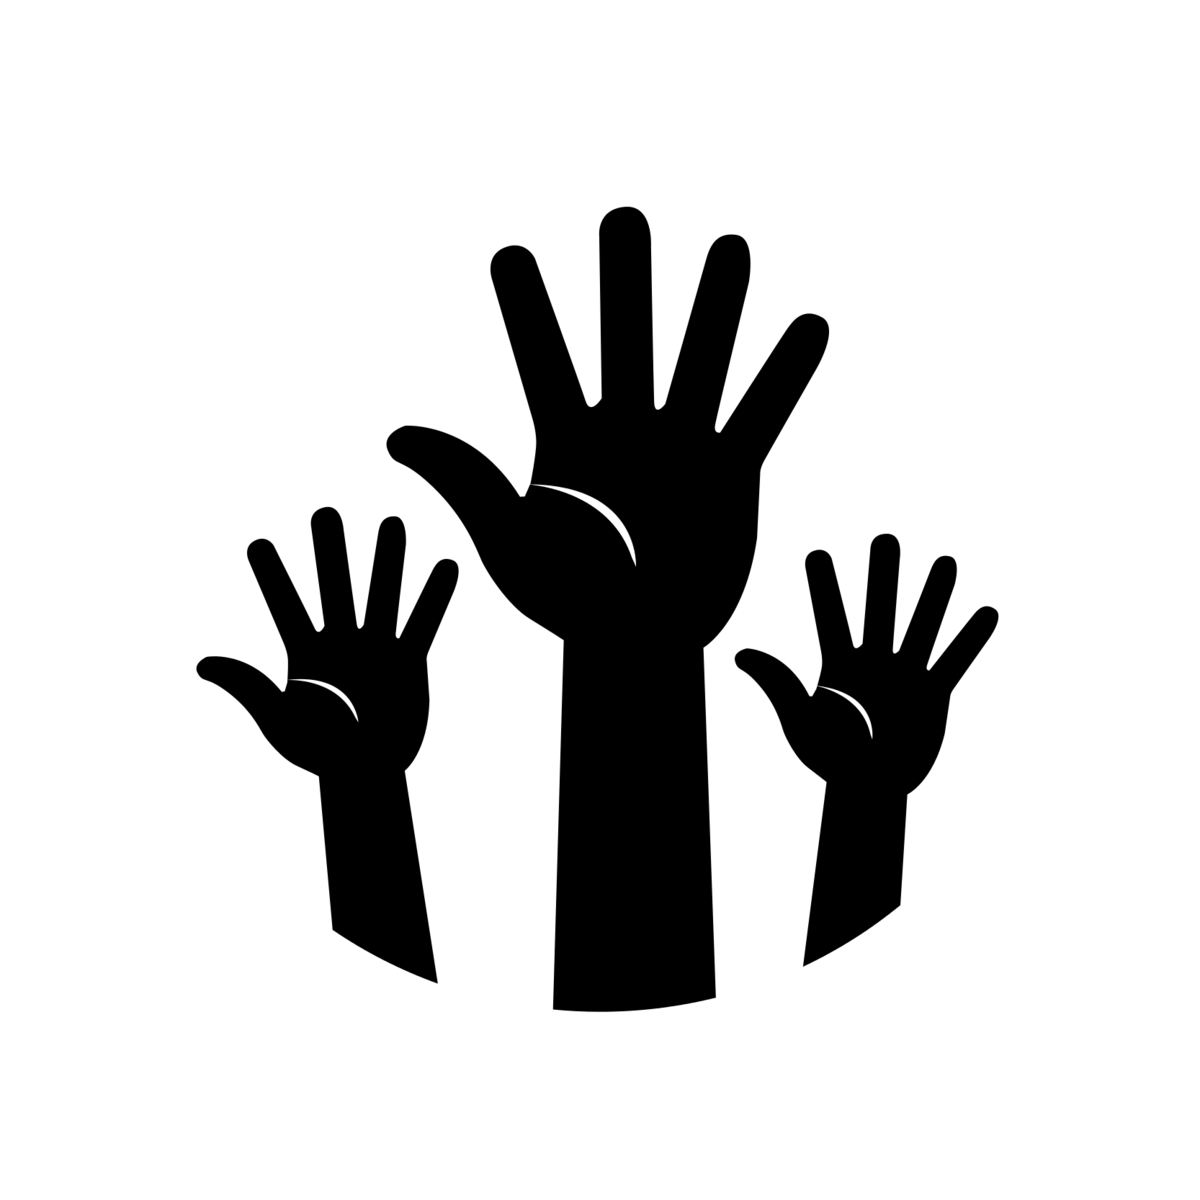
\includegraphics[height=1.5em]{images/hands}}
\newcommand{\transpose}[0]{{\textrm{\tiny{\sf{T}}}}}
\newcommand{\norm}{{\mathcal{N}}}
\newcommand{\cutoff}[0]{\kappa}
\newcommand{\instD}[0]{\dataset}
\newcommand{\insts}[0]{\mathcal{I}}
\newcommand{\inst}[0]{i}
\newcommand{\instI}[1]{i^{(#1)}}

% Iteration specific instance of variable/function/anything
% Introduced in the BO section, but moved up here to make it available within other macros
\newcommand{\iter}[2][\bocount]{{#2}^{(#1)}}

%--------HPO parameter macros-----------

% Parameter Configuration Space
\newcommand{\pcs}[0]{\pmb{\Lambda}}

% ???
\newcommand{\bx}[0]{\conf}

% Parameter Configuration
\newcommand{\conf}[0]{\pmb{\lambda}}

% Final Configuration
\newcommand{\finconf}[0]{\pmb{\hat{\lambda}}}

% Configuration corresponding to a given iteration -- better use \iter!
\newcommand{\confI}[1]{{\conf}^{(#1)}}

% Default Configuration
\newcommand{\defconf}[0]{{\conf}_{\text{def}}}

% Incumbent Configuration
\newcommand{\incumbent}[1][\bocount]{\iter[#1]{\finconf}}

% Optimal Configuration
\newcommand{\optconf}[0]{{\conf}^*}

% Configuration Space
\newcommand{\confs}[0]{\pcs}

%----------------------------------------

%\newcommand{\vlambda}[0]{\bm{\lambda}}
%\newcommand{\vLambda}[0]{\bm{\Lambda}}
\newcommand{\dataset}[0]{\mathcal{D}}
\newcommand{\datasets}[0]{\mathbf{D}}
\newcommand{\loss}[0]{L}
\newcommand{\risk}{\mathcal{R}}
\newcommand{\riske}{\mathcal{R}_{\text{emp}}}
\newcommand{\cost}[0]{c}
\newcommand{\costI}[1]{c^{(#1)}}

% Gaussian Process
\newcommand{\gp}{\mathcal{G}}
% Family of Objective Functions
\newcommand{\objF}{F}

%---------------BO Macros------------------

% BO loop counter
\newcommand{\bocount}{t}
% BO loop counter max, the counter runs from 1 to this value
\newcommand{\bobudget}{T}
% BO loop observation
\newcommand{\obs}[1][\conf]{\cost({#1})}
% BO loop observation space
\newcommand{\obsspace}{\mathcal{Y}}
% BO loop next observation
\newcommand{\bonextobs}{\obs[\iter{\conf}]}
% Acquisition Function, no args
\newcommand{\acq}{u}
% Standard Normal PDF
\newcommand{\pdf}{\phi}
% Standard Normal CDF
\newcommand{\cdf}{\Phi}
% Mean
\newcommand{\mean}{\mu}
% Standard Deviation
\newcommand{\stddev}{\sigma}
% Variance
\newcommand{\variance}{\sigma^2}
% Noise
\newcommand{\noise}{\nu}
% BO loop next selected sample
\newcommand{\bonextsample}{\confI{\bocount}}

% Single hyperparameter
\newcommand{\hyperparam}{\lambda}

% Single hyperparameter within a hyperparameter configuration
\newcommand{\hyperparami}[1][i]{{\hyperparam}_#1}

% Full definition of final configuration
\newcommand{\finconffull}{\incumbent[\bobudget]}

% Dataset
\newcommand{\datasetHPO}{{\dataset}_{HPO}}

% Dataset definition
\newcommand{\datasetHPOdef}{{\langle \bonextsample,\,\bonextobs \rangle}_{\bocount=1}^{\bobudget}}

% Double Display Fraction, forces large displays for everything in numerator and denominator
\newcommand\ddfrac[2]{\frac{\displaystyle #1}{\displaystyle #2}}

% Conditional Probability "Given That" Relation, source:https://tex.stackexchange.com/a/141685/205886
\newcommand\given[1][]{\:#1\vert\:}

% Expectation as a math operator
\DeclareMathOperator*{\E}{\mathbb{E}}

% Citation 
\newcommand{\source}[1]{
    \begin{flushright}
    	Source: \lit{#1}
    \end{flushright}
}
%-------------------------------------------

%Real numbers set
\newcommand{\realnum}{\mathbb{R}}
%Configuration space - do not use
%\newcommand{\configspace}{\Theta}
%Instances - do not use
%\newcommand{\instances}{\mathcal{I}}
%Expected value
\newcommand{\expectation}{\mathbb{E}}
%Kernel
\newcommand{\kernel}{\kappa}
%Constraint function
\newcommand{\constraintf}{c}
%Normal distribution
\newcommand{\normaldist}{\mathcal{N}}

% \renewcommand{\vec}[1]{\mathbf{#1}}
\newcommand{\hist}[0]{\dataset_{\text{Hist}}}
\newcommand{\param}[0]{p}
\newcommand{\algo}[0]{\mathcal{A}}
\newcommand{\algos}[0]{\mathbf{A}}
%\newcommand{\nn}[0]{N}
\newcommand{\feats}[0]{\mathcal{X}_{\text{meta}}}
\newcommand{\feat}[0]{\x_{\text{meta}}}
%\newcommand{\cluster}[0]{\vec{h}}
%\newcommand{\clusters}[0]{\vec{H}}
\newcommand{\perf}[0]{\mathbb{R}}
%\newcommand{\surro}[0]{\mathcal{S}}
\newcommand{\surro}[0]{\hat{\cost}}
\newcommand{\func}[0]{f}
\newcommand{\epm}[0]{\surro}
\newcommand{\portfolio}[0]{\mathbf{P}}
\newcommand{\schedule}[0]{\mathcal{S}}

% Machine Learning
\newcommand{\mdata}[0]{\dataset_{\text{meta}}}
\newcommand{\datasettrain}[0]{\dataset_{\text{train}}}
\newcommand{\datasetval}[0]{\dataset_{\text{val}}}
\newcommand{\datasettest}[0]{\dataset_{\text{test}}}
\newcommand{\x}[0]{\mathbf{x}}
\newcommand{\y}[0]{y}
\newcommand{\xI}[1]{\mathbf{x}^{(#1)}}
\newcommand{\yI}[1]{y^{(#1)}}
\newcommand{\fx}{f(\mathbf{x})}  % f(x), continuous prediction function
\newcommand{\Hspace}{\mathcal{H}} % hypothesis space where f is from
\newcommand{\fh}{\hat{f}}       % f hat, estimated prediction function

% Deep Learning
\newcommand{\weights}[0]{\theta}
\newcommand{\metaweights}[0]{\phi}


% reinforcement learning
\newcommand{\policies}[0]{\mathbf{\Pi}}
\newcommand{\policy}[0]{\pi}
\newcommand{\actionRL}[0]{a}
\newcommand{\stateRL}[0]{s}
\newcommand{\statesRL}[0]{\mathcal{S}}
\newcommand{\rewardRL}[0]{r}
\newcommand{\rewardfuncRL}[0]{\mathcal{R}}

\RestyleAlgo{algoruled}
\DontPrintSemicolon
\LinesNumbered
\SetAlgoVlined
\SetFuncSty{textsc}

\SetKwInOut{Input}{Input}
\SetKwInOut{Output}{Output}
\SetKw{Return}{return}

%\newcommand{\changed}[1]{{\color{red}#1}}

%\newcommand{\citeN}[1]{\citeauthor{#1}~(\citeyear{#1})}

\renewcommand{\vec}[1]{\mathbf{#1}}
\DeclareMathOperator*{\argmin}{arg\,min}
\DeclareMathOperator*{\argmax}{arg\,max}

%\newcommand{\aqme}{\textit{AQME}}
%\newcommand{\aslib}{\textit{ASlib}}
%\newcommand{\llama}{\textit{LLAMA}}
%\newcommand{\satzilla}{\textit{SATzilla}}
%\newcommand{\satzillaY}[1]{\textit{SATzilla'{#1}}}
%\newcommand{\snnap}{\textit{SNNAP}}
%\newcommand{\claspfolioTwo}{\textit{claspfolio~2}}
%\newcommand{\flexfolio}{\textit{FlexFolio}}
%\newcommand{\claspfolioOne}{\textit{claspfolio~1}}
%\newcommand{\isac}{\textit{ISAC}}
%\newcommand{\eisac}{\textit{EISAC}}
%\newcommand{\sss}{\textit{3S}}
%\newcommand{\sunny}{\textit{Sunny}}
%\newcommand{\ssspar}{\textit{3Spar}}
%\newcommand{\cshc}{\textit{CSHC}}
%\newcommand{\cshcpar}{\textit{CSHCpar}}
%\newcommand{\measp}{\textit{ME-ASP}}
%\newcommand{\aspeed}{\textit{aspeed}}
%\newcommand{\autofolio}{\textit{AutoFolio}}
%\newcommand{\cedalion}{\textit{Cedalion}}
\newcommand{\fanova}{\textit{fANOVA}}
\newcommand{\sbs}{\textit{SB}}
\newcommand{\oracle}{\textit{VBS}}

% like approaches
\newcommand{\claspfoliolike}[1]{\texttt{claspfolio-#1-like}}
\newcommand{\satzillalike}[1]{\texttt{SATzilla'#1-like}}
\newcommand{\isaclike}{\texttt{ISAC-like}}
\newcommand{\ssslike}{\texttt{3S-like}}
\newcommand{\measplike}{\texttt{ME-ASP-like}}

\newcommand{\irace}{\textit{I/F-race}}
\newcommand{\gga}{\textit{GGA}}
\newcommand{\smac}{\textit{SMAC}}
\newcommand{\paramils}{\textit{ParamILS}}
\newcommand{\spearmint}{\textit{Spearmint}}
\newcommand{\tpe}{\textit{TPE}}


\usepackage{pifont}
\newcommand{\itarrow}{\mbox{\Pisymbol{pzd}{229}}}
\newcommand{\ithook}{\mbox{\Pisymbol{pzd}{52}}}
\newcommand{\itcross}{\mbox{\Pisymbol{pzd}{56}}}
\newcommand{\ithand}{\mbox{\raisebox{-1pt}{\Pisymbol{pzd}{43}}}}

%\DeclareMathOperator*{\argmax}{arg\,max}

\newcommand{\ie}{{\it{}i.e.\/}}
\newcommand{\eg}{{\it{}e.g.\/}}
\newcommand{\cf}{{\it{}cf.\/}}
\newcommand{\wrt}{\mbox{w.r.t.}}
\newcommand{\vs}{{\it{}vs\/}}
\newcommand{\vsp}{{\it{}vs\/}}
\newcommand{\etc}{{\copyedit{etc.}}}
\newcommand{\etal}{{\it{}et al.\/}}

\newcommand{\pscProc}{{\bf procedure}}
\newcommand{\pscBegin}{{\bf begin}}
\newcommand{\pscEnd}{{\bf end}}
\newcommand{\pscEndIf}{{\bf endif}}
\newcommand{\pscFor}{{\bf for}}
\newcommand{\pscEach}{{\bf each}}
\newcommand{\pscThen}{{\bf then}}
\newcommand{\pscElse}{{\bf else}}
\newcommand{\pscWhile}{{\bf while}}
\newcommand{\pscIf}{{\bf if}}
\newcommand{\pscRepeat}{{\bf repeat}}
\newcommand{\pscUntil}{{\bf until}}
\newcommand{\pscWithProb}{{\bf with probability}}
\newcommand{\pscOtherwise}{{\bf otherwise}}
\newcommand{\pscDo}{{\bf do}}
\newcommand{\pscTo}{{\bf to}}
\newcommand{\pscOr}{{\bf or}}
\newcommand{\pscAnd}{{\bf and}}
\newcommand{\pscNot}{{\bf not}}
\newcommand{\pscFalse}{{\bf false}}
\newcommand{\pscEachElOf}{{\bf each element of}}
\newcommand{\pscReturn}{{\bf return}}

%\newcommand{\param}[1]{{\sl{}#1}}
\newcommand{\var}[1]{{\it{}#1}}
\newcommand{\cond}[1]{{\sf{}#1}}
%\newcommand{\state}[1]{{\sf{}#1}}
%\newcommand{\func}[1]{{\sl{}#1}}
\newcommand{\set}[1]{{\Bbb #1}}
%\newcommand{\inst}[1]{{\tt{}#1}}
\newcommand{\myurl}[1]{{\small\sf #1}}

\newcommand{\Nats}{{\Bbb N}}
\newcommand{\Reals}{{\Bbb R}}
\newcommand{\extset}[2]{\{#1 \; | \; #2\}}

\newcommand{\vbar}{$\,\;|$\hspace*{-1em}\raisebox{-0.3mm}{$\,\;\;|$}}
\newcommand{\vendbar}{\raisebox{+0.4mm}{$\,\;|$}}
\newcommand{\vend}{$\,\:\lfloor$}


\newcommand{\goleft}[2][.7]{\parbox[t]{#1\linewidth}{\strut\raggedright #2\strut}}
\newcommand{\rightimage}[2][.3]{\mbox{}\hfill\raisebox{1em-\height}[0pt][0pt]{\includegraphics[width=#1\linewidth]{#2}}\vspace*{-\baselineskip}}





\title[AutoML: Local Importance]{AutoML: Interpretability}
\subtitle{Incumbent Analysis and Local Hyperparameter Importance}
\author[Marius Lindauer]{Bernd Bischl \and Frank Hutter \and Lars Kotthoff\newline \and \underline{Marius Lindauer} \and Joaquin Vanschoren}
\institute{}
\date{}


% \AtBeginSection[] % Do nothing for \section*
% {
%   \begin{frame}{Outline}
%     \bigskip
%     \vfill
%     \tableofcontents[currentsection]
%   \end{frame}
% }

\begin{document}
	
	\maketitle
	

%----------------------------------------------------------------------
%----------------------------------------------------------------------
\begin{frame}[c,fragile]{Idea}

\begin{center}
\scalebox{0.9}{
    \let\oldpause=\pause \def\pause{} 
	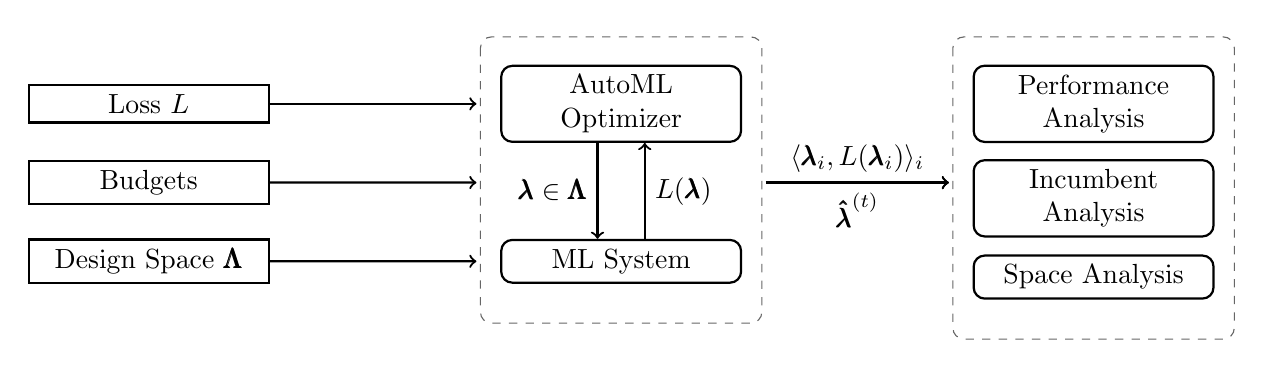
\begin{tikzpicture}[node distance=4cm, thick]
	\node (function) [data] {Loss $\loss$};
	\node (budgets) [data, below of=function, node distance=1cm] {Budgets};
	\node (space) [data, below of=budgets, node distance=1cm] {Design Space $\pcs$};
	
	\pause
	\node (hb) [activity, right of=space, node distance=6cm, yshift=-0.0cm] {ML System};
	\node (kde) [activity, above of=hb, node distance=2cm] {AutoML Optimizer};
	
	\draw[myarrow] ($(kde.south)+(-0.3,0.0)$) -- ++(0.0,-0.6) node[left] {$\conf \in \pcs$} -- ($(hb.north)+(-0.3,+0.0)$);
	\draw[myarrow] ($(hb.north)+(0.3,+0.0)$) -- ++(0.0,0.6) node[right] {$\loss(\conf)$} -- ($(kde.south)+(0.3,0.0)$);
	
	\draw[myarrow] (function.east) -- ($(kde.west)+(-0.3,0.0)$);
	\draw[myarrow] (budgets.east) -- ($(kde.west)+(-0.3,-1.)$);
	\draw[myarrow] (space.east) -- ($(kde.west)+(-0.3,-2.)$);
	
	\pause
	\node (perf) [activity, right of=kde, node distance=6cm] {Performance Analysis};
	\node (budget) [activity, below of=perf, node distance=1.2cm] {Incumbent Analysis};
	\node (imp) [activity, below of=budget, node distance=1cm] {Space Analysis};
	
	\draw[myarrow] ($(kde.east)+(0.3,-1.)$) -- node[above] {$\langle \conf_i, \loss(\conf_i)\rangle_i$} ($(perf.west)+(-0.3,-1.)$);
	\draw[myarrow] ($(kde.east)+(0.3,-1.)$) -- node[below] {$\incumbent$} ($(perf.west)+(-0.3,-1.)$);
	
	\begin{pgfonlayer}{background}
	
	% Configuration Process
	\path (kde -| kde.west)+(-0.25,0.85) node (resUL) {};
	\path (hb.east |- hb.south)+(0.25,-0.5) node(resBR) {};
	\path [rounded corners, draw=black!60, dashed] (resUL) rectangle (resBR);
	\path (hb.east |- hb.south)+(-.5,-.3) node [text=black!60] {};
	
	\path (perf -| perf.west)+(-0.25,0.85) node (resUL) {};
	\path (imp.east |- imp.south)+(0.25,-0.5) node(resBR) {};
	\path [rounded corners, draw=black!60, dashed] (resUL) rectangle (resBR);
	\path (imp.east |- imp.south)+(-.5,-.3) node [text=black!60] {};
	
	\end{pgfonlayer}

\end{tikzpicture}
	\let\pause=\oldpause
}
\end{center}

\begin{itemize}
	\item[$\leadsto$] focus on why is the eventually returned configuration a good choice
\end{itemize}

\end{frame}
%-----------------------------------------------------------------------
%----------------------------------------------------------------------
\begin{frame}[c]{Local Importance \litw{\href{https://www.tnt.uni-hannover.de/papers/data/1410/18-LION12-CAVE.pdf}{Biedenkapp et al. 2018}}}

\begin{columns}
	
	\column{0.4\textwidth}
	\begin{center}
		% Created by Katha as part of the BOBO Paper
		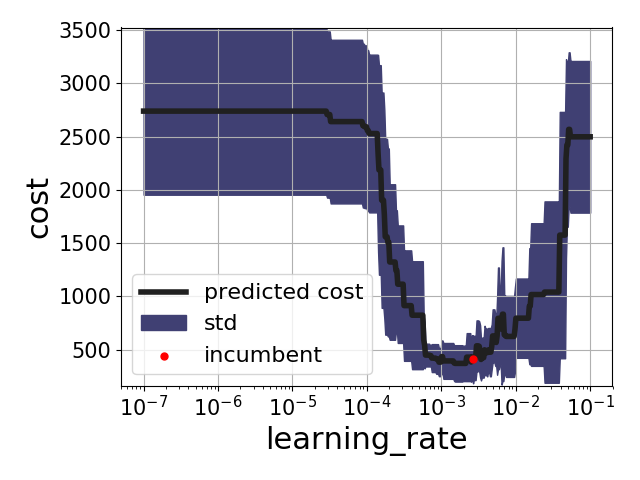
\includegraphics[width=1.0\textwidth]{images/learning_rate_lpi.png}\\
		Source: \lit{\href{https://arxiv.org/pdf/1908.06674.pdf}{Lindauer et al. 2019}}
	\end{center}
	
	\column{0.6\textwidth}
	
	\begin{itemize}
		\item Typical question of users:
		\begin{itemize}
			\item How would the performance change\\
			if we change hyperparameter $\conf_i$?
		\end{itemize}
        \pause 
		\item Problem: Running full study is often too expensive
		\begin{itemize}
			\item Each run of an ML-system is potential expensive
		\end{itemize}
		\pause
		\item \alert{Key Ideas:}
		\begin{itemize}
			\item Re-use probabilistic models as trained in BO
			\item Plot performance change around $\incumbent$\\
			 along each dimension
		\end{itemize} 
	\end{itemize}
	
\end{columns}

\end{frame}
%-----------------------------------------------------------------------
%----------------------------------------------------------------------
\begin{frame}[c]{Quantifying Local Importance \litw{\href{https://www.tnt.uni-hannover.de/papers/data/1410/18-LION12-CAVE.pdf}{Biedenkapp et al. 2018}}}

\begin{eqnarray}
\text{VAR}_{\conf} (i)  &=& \sum_{v \in \pcs_{i}} (\mathbb{E}_{v \sim \pcs_{i}}[\loss(\conf) ] - \loss(\conf[ \conf_{i} := v]))^2\\
\pause
\text{LPI}( i  \mid \conf ) &=& \frac{VAR_{\conf} (i) }{ \sum_{j}  VAR_{\conf} (j)}
\end{eqnarray}

\bigskip
\pause

\begin{itemize}
	\item[$\leadsto$] While fixing all other hyperparameters to the incumbent value,\\ the hyperparameter with the highest variance  is the most important one
\end{itemize}

\end{frame}
%-----------------------------------------------------------------------
%----------------------------------------------------------------------
\begin{frame}[c]{Ablation Study for Importance}

\begin{itemize}
	\item Users often start from some kind of default configuration
	\begin{enumerate}
		\item As given in the documentation 
		\item Or as always used in the last time
	\end{enumerate}
    \pause
	\item \alert{Key Idea}: Going from the default to the automatically optimized configuration,\\
	 which choices where important?
\end{itemize}

\begin{eqnarray}
\confI{\text{start}} &=& [1, 1, 0, 100]  \nonumber\\
\confI{\text{end}} &=& [0.98, 2.42, 1, 42]  \nonumber
\end{eqnarray}

\pause
\begin{itemize}
	\item Cheap approach: Assess $\confI{\text{end}}$ with each hyperparameter value from $\confI{\text{start}}$
	\pause
	\item Expensive approach: Try all mixtures of $\confI{\text{end}}$ and $\confI{\text{start}}$
	\begin{itemize}
		\item  Only feasible for small spaces and fairly cheap ML systems
	\end{itemize}
	\pause
	\item Trade-off: Find a way from $\confI{\text{start}}$ to $\confI{\text{end}}$ in a greedy fashion \lit{\href{https://link.springer.com/article/10.1007\%2Fs10732-014-9275-9}{Fawcett and Hoos 2016}}
\end{itemize}

\end{frame}
%-----------------------------------------------------------------------
%----------------------------------------------------------------------
\begin{frame}[c]{Greedy Ablation Study}

Given:
\begin{eqnarray}
\begin{array}{lll}
\confI{\text{start}} &= [1, 1, 0, 100] & \loss_{\text{start}} = 20\% \nonumber\\
\confI{\text{end}} &= [0.98, 2.42, 1, 42]  & \loss_{\text{end}} = 4\% \nonumber
\end{array}
\end{eqnarray}

\pause
1st Iteration:
\begin{eqnarray}
\begin{array}{lll}
\confI1& = [\alert{0.98}, 1, 0, 100] & \loss_1 = 19\% \nonumber\\
\pause
\confI2 &= [1, \alert{2.42}, 0, 100] & \loss_2 = 20\% \nonumber\\
\pause
\confI3 &= [1, 1, \alert{1}, 100] & \loss_3 = 7\% \nonumber\\
\pause
\confI4 &= [1, 1, 0, \alert{42}] & \loss_4 = 16\% \nonumber\\
\end{array}
\end{eqnarray}

\pause
$\leadsto$ 1st step: $\conf_2$ -- flipping hyperparameter 3


\end{frame}
%-----------------------------------------------------------------------
%----------------------------------------------------------------------
\begin{frame}[c]{Greedy Ablation Study}

Given:
\begin{eqnarray}
\begin{array}{lll}
\confI{\text{start}} &= [1, 1, 0, 100] & \loss_{\text{start}} = 20\% \nonumber\\
\confI{s1} &= [1, 1, \alert{1}, 100]  & \loss = 7\% \nonumber\\
\confI{\text{end}} &= [0.98, 2.42, 1, 42]  & \loss_{\text{end}} = 4\% \nonumber
\end{array}
\end{eqnarray}

2nd Iteration:
\begin{eqnarray}
\begin{array}{ll}
\confI1 = [\alert{0.98}, 1, 1, 100] & \loss_1 = 6\% \nonumber\\
\pause
\confI2 = [1, \alert{2.42}, 1, 100] & \loss_2 = 7\% \nonumber\\
\pause
\confI3 = [1, 1, 1, \alert{42}] & \loss_3 = 5\% \nonumber\\
\end{array}
\end{eqnarray}

$\leadsto$ 2nd step: $\conf_3$ -- flipping hyperparameter 4

\end{frame}
%-----------------------------------------------------------------------
%----------------------------------------------------------------------
\begin{frame}[c]{Greedy Ablation Study}

Given:
\begin{eqnarray}
\begin{array}{lll}
\confI{\text{start}} &= [1, 1, 0, 100] & \loss_{\text{start}} = 20\% \nonumber\\
\confI{s1} &= [1, 1, \alert{1}, 100]  & \loss = 7\% \nonumber\\
\confI{s2} &= [1, 1, 1, \alert{42}]  & \loss = 5\% \nonumber\\
\confI{\text{end}} &= [0.98, 2.42, 1, 42]  & \loss_{\text{end}} = 4\% \nonumber
\end{array}
\end{eqnarray}

3rd Iteration:
\begin{eqnarray}
\begin{array}{ll}
\confI1 = [\alert{0.98}, 1, 1, 100] & \loss_1 = 4\% \nonumber\\
\confI2 = [1, \alert{2.42}, 1, 100] & \loss_2 = 5\% \nonumber\\
\end{array}
\end{eqnarray}

$\leadsto$ 2nd step: $\conf_3$ -- flipping hyperparameter 1

\end{frame}
%-----------------------------------------------------------------------
%----------------------------------------------------------------------
\begin{frame}[c]{Greedy Ablation Study}

Ablation Path:
\begin{eqnarray}
\begin{array}{ll}
\confI{\text{start}} = [1, 1, 0, 100] & \loss_{\text{start}} = 20\% \nonumber\\
\confI{s1} = [1, 1, \alert{1}, 100]  & \loss = 7\% \nonumber\\
\confI{s1} = [1, 1, 1, \alert{42}]  & \loss = 5\% \nonumber\\
\confI{s3} = [\alert{0.98}, 1, 1, 42] & \loss = 4\% \nonumber\\
\confI{s4} = [0.98, \alert{2.42}, 1, 42] & \loss = 4\% \nonumber\\
\confI{\text{end}} = [0.98, 2.42, 1, 42]  & \loss_{\text{end}} = 4\% \nonumber
\end{array}
\end{eqnarray}

\end{frame}
%-----------------------------------------------------------------------
%----------------------------------------------------------------------
\begin{frame}[c,fragile]{Greedy Ablation Pseudo Code}

\LinesNotNumbered
\begin{algorithm}[H]
	\Input{%
		Algorithm $\algo$ with configuration space $\confs$,
		start configuration $\confI{\text{start}}$,\\
		end configuration $\confI{\text{end}}$, cost metric $\cost$
	}
	\BlankLine
	$\conf \leftarrow  \confI{\text{start}}$; \\
	$P \leftarrow [] $ ;\\ 
	\pause
	\ForEach{$\bocount \in \{1 \ldots |\pcs|\}$}{
		\pause
		\ForEach{$\delta \in \Delta(\conf, \confI{\text{end}})$}{
			$\conf'_\delta$ $\leftarrow$ apply $\delta$ to $\conf$;\\
			evaluate $\cost(\conf'_\delta)$;
		}
	  \pause
		Determine most important change $\delta^* \in \argmin_{\delta \in \Delta(\conf, \confI{\text{end}})} \cost(\conf_\delta)$;\\
		$\conf$ $\leftarrow$ apply $\delta^*$ to $\conf$;\\
		P.append($\delta^*$);
	}
	\pause
	\Return{Ablation path $P$}
	\caption{Greedy Ablation}
	\end{algorithm}
	
\end{frame}
%----------------------------------------------------------------------
%----------------------------------------------------------------------
\begin{frame}[c,fragile]{Remarks on Ablation}

\begin{itemize}
	\item Even this greedy ablation requires $\mathcal{O}(n^2)$ steps 
	\pause
	\item[$\leadsto$] We can also speedup that up by using surrogate models\\
	\lit{\href{https://www.tnt.uni-hannover.de/papers/data/1396/17-AAAI-Surrogate-Ablation.pdf}{Biedenkapp et al. 2017}}
	\medskip
	\pause
	\item Common observations:
	\begin{enumerate}
		\item Some hyperparameters might not matter ($\conf_{2}$ in the example)
		\pause
		\item Often only a few of the hyperparameters have an big impact
		\pause
		\item You have plateaus in your ablation path because of interaction effects
	\end{enumerate}
\end{itemize}

\end{frame}
%----------------------------------------------------------------------


%-----------------------------------------------------------------------
\end{document}
